\section{Auswahl der Technologie - Client}
\setauthor{David Hauser}

\subsection{Unterschied Framework und Library}
\subsection{Technologie zur Entwicklung des Frontends}
\subsection{Angular}
\subsection{React}

\section{Auswahl der Technologie - Datenbank[SK]}
\setauthor{Simon Koll}
Die Datenbank spielt für das Projekt eine sehr wichtige Rolle, daher wurden hier folgende Kriterien aufgestellt:

\begin{itemize}
  \item Das Projekt besteht aus Hard- und Software, die Daten sowohl abspeichern als auch abfragen. Das kann je nach Anwendungsfall unterschiedlich sein.
  \item Vom Dashboard können beispielsweise Kennzeichen mit Gültigkeitsdauer, aber auch nur einfache NFC-Codes gesendet werden.
  \item In der Zukunft soll die Möglichkeit bestehen, weitere Zutrittsmöglichkeit hinzuzufügen. Daher muss sich die Datenbank der sich ändernden Datenstruktur anpassen können.
\end{itemize}

\subsection{Relationale Datenbanken}

Das Team befand sich nun vor der Entscheidung, ein relationales Datenbanksystem zu verwenden, oder ein nicht relationales Datenbanksystem. \\
Die größten Unterschiede hierbei sind, dass bei relationalen SQL-Datenbanken den gespeicherten Daten Tabellen vorgegeben sind, das sogenannte Schema. Das ist bei NoSQL-Datenbanken ebenfalls möglich, jedoch optional.\\
Relationale Datenbanken verfolgen das ACID-Prinzip. ACID steht für

\begin{itemize}
  \item \textit{Atomicity}
  \subitem Alle Änderungen der Datenbank werden als einzige Operation verarbeitet. Entweder werden alle Änderungen wie Inserts, Updates usw. durchgeführt, oder keine davon.
  \item \textit{Consistency}
  \subitem Zu Beginn und zum Ende jeder Transaktion sind die Daten konsistent. Wenn man als Beispiel eine Geldüberweisung darstellt, ist bei "Consistency" die Gesamtsumme der Geldmittel auf beiden Konten am Anfang und am Ende jeder Transaktion gleich.
  \item \textit{Isolation}
  \subitem Andere Transaktionen haben keine Einsicht in die Transaktion. Isolation bedeutet also, dass parallel laufende Transaktionen sich wie serialisierte verhalten.
  \item \textit{Durability}
  \subitem Die Daten bleiben nach Ende der Transaktion bestehen und auch bei einem kompletten Systemausfall nicht revidiert.
\end{itemize}
\cite{ACID}

\subsection{MongoDB}
Das Team entschied sich für eine der bekanntesten NoSQL-Datenbanken, \textbf{MongoDB}. Diese bietet einige Vorteile gegenüber den relationalen SQL-Datenbanken:

\begin{itemize}
  \item \textit{Skalierbarkeit}
  \item \textit{Verfügbarkeit}
  \item \textit{Flexibilität}
\end{itemize}
\cite{VorteileMongoDB}
\section{Auswahl der Technologie - Kennzeichenerkennung[SK]}
\setauthor{Simon Koll}
Das Herz von APERTA ist die Kennzeichenerkennung. Dieses Alleinstellungsmerkmal separiert das Projekt von möglicher Konkurrenz. Um eine schnelle, und problemfreie Lösung zu liefern, versuchte das Team, eine für österreichische Kennzeichen optimierte Lösung zu implementieren. 

\section{Auswahl der Technologie - Backend[SK]}
\setauthor{Simon Koll}
\subsection{Anforderungen an das Backend}
Für das Backend kamen mehrere Technologien in Frage, wie unter anderem Java, JavaScript, Python, PHP, C$\sharp$, und viele mehr.
Um das Backend zu realisieren, muss die Technologie einige bestimmte Eigenschaften besitzen.\cite{CompareBackendLanguage}
\begin{itemize}
    \item \textit{Java:} 
    \subitem Die Vorteile von Java liegen in der Fehlerbehandlung, sowie in Bereichen wie Multithreading und Performanz. Die strikte Fehlerbehandlung führt dabei aber zum Verlust von Flexibilität und Kompaktheit des Codes.
    \item \textit{JavaScript:} 
    \subitem Die Syntax von JavaScript ähnelt der von Java. Entwickelt als Scripting-Sprache für HTML, ist JavaScript einfach zu lernen und zu benutzen. Bei der Entwicklung von Websites kann JavaScript direkt in den Quellcode der HTML-Seite eingearbeitet werden. Aber auch im Backend-Bereich kann mit NodeJS in JavaScript entwickelt werden.
    \item \textit{Python:}
    \subitem Python ist eine der mit Abstand am leichtesten zu lesenden Programmiersprachen. Die flache Hierarchie ermöglicht ein einfaches Verständnis von Programmen und Codestücken. Weiters macht Python den Entwickler auf jeden Fehler aufmerksam, wenn dieser nicht ausdrücklich ignoriert werden soll.
    Jedoch ist Python manchmal langsamer in der Ausführung als die konkurrierenden Sprachen. Zusätzlich ist durch die Verwendung von Leerzeichen zur Einrückung ein häufiger Fehlergrund hinzugekommen.
    \item \textit{PHP:} 
    \subitem Die PHP Syntax erinnert an eine Mischung aus C, Java und Perl. Das Ziel von PHP ist es, Entwickler schnell und einfach dynamisch generierte Webpages zu bauen. Die vermischte Syntax ist jedoch etwas chaotisch, darum ist es leicht sich in falschen Angewohnheiten zu verirren und Sicherheitslücken offen zu lassen.
  \end{itemize}
  Aufgrund vorhandener Vorkenntnisse standen für das Team 3 der oben genannten Technologien zur Auswahl:

  \begin{itemize}
    \item Java,
    \item JavaScript und
    \item Python
  \end{itemize}

  \subsection{Verwendung von NodeJS}
  Von diesen konnte sich JavaScript durchsetzen. Die Gründe dafür waren:\cite{WhyNodeJs}
  \begin{itemize}
    \item NPM:
    Der NPM oder \textit{Node Package Manager}, ist ein Paketmanager für JavaScript, welcher bei NodeJS standardmäßig mitgeliefert wird. Bei NPM werden wiederverwendbare Programmteilen veröffentlicht. Diese können mittels des NPM eingenen Command Line Interfaces installiert werden. Weiters bietet der NPM eine integrierte Versionsverwaltung der Pakete sowie eine Verwaltung der Abhängigkeiten.
    In diesem Projekt wurden beispielsweise die Module \textit{express} und \textit{mongodb} verwendet. 
    \linebreak
    \textit{express} ist ein Framework, welches vor allem in NodeJS Projekten verwendet wird. Die Vorteile von Express sind unter anderem die dem Team bereits bekannte Programmiersprache JavaScript, die Unterstützung der Google V8 engine für bessere Performance, die Robustheit bei einer Vielzahl an HTTP-Anfragen, sowie die einfache Einbindung weiterer Module und Drittanbieterapplikationen. \cite{WhyExpress}
    \linebreak
    \linebreak
    \textit{mongodb} stellt dem Entwickler eine API zur Verfügung, welche die Nutzung einer MongoDB-Datenbank stark vereinfacht.
    \item Verwendung einer NoSQL Datenbank:
    Aufgrund des Formates, mit dem die Daten aus dem Frontend kommen, bat sich eine nicht relationale Datenbank für das Team an. Die dokumentenorientierte Datenbank MongoDB ist bekannt für ihre hohe Verfügbarkeit, sowie die gute Skalierbarkeit.\cite{WhyMongoDB}
    \linebreak
    \item Behandlung von JSON:
    NodeJS zeichnet sich durch seine einfach Verwendung von JSON-Daten aus. Diese können ohne Parsing oder andere Konvertierungen verarbeitet und darauf zugegriffen werden. Dank NodeJS können JSON Objekte mittels REST-API Anfragen direkt für den Client bereitgestellt werden.
    Danke NodeJS kann eine Einfache Verbindung zwischen Frontend-Clients und dem Backend-Server geschaffen werden.
  \end{itemize}

\section{Auswahl der Technologie - Hardware[SK]}
\setauthor{Simon Koll}
\subsection{Anforderungen an die Hardware}
Das Projekt sollte so vielseitig wie möglich, jedoch auch so kompakt wie möglich sein. Dazu musste auf kleine Komponenten gesetzt werden. Diese soll dennoch leistungsfähig genug sein, um jede der drei Zugangsmöglichkeiten parallel zu verwalten.
\subsubsection{Raspberry Pi}
Die Wahl des Herzstückes fiel auf einen Raspberry Pi.
Der Raspberry Pi ist ein vollwertiger Computer, welcher etwas größer als eine Kreditkarte ist. Er besitzt alle bekannten Anschlüsse eines normalgroßen PCs, wie HDMI-Ausgänge für Monitore, USB-Ports für Peripherie wie Maus, Tastatur oder Webcams, sowie einen LAN-Port für eine kabelgebundene Netzwerkverbindung.
Als Betriebssystem des Raspberry Pi wurde das vom Hersteller empfohlene Raspbian OS verwendet. Dieses bietet eine grafische Benutzeroberfläche, sowie die Möglichkeit den Raspberry auch ohne angeschlossenen Monitor betreiben zu können. \cite{WhatIsRaspberryPi}
\begin{figure}[h]
  \centering
  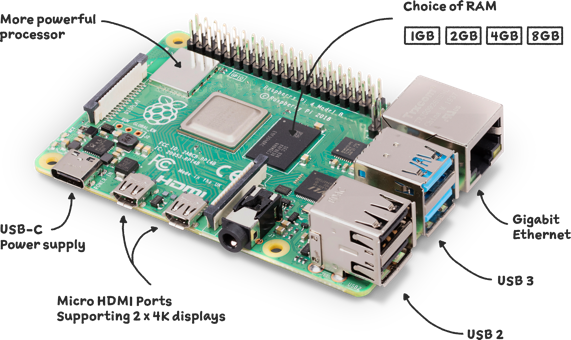
\includegraphics[width=8cm]{pics/raspberry-pi-4-labelled-dc5d034fb85873018dff0857352b40bf.png}
  \end{figure}
\cite{RaspberryImage}

Auszeichnungsmerkmale des Raspberry Pi sind unter anderem die geringen Anschaffungskosten von ab 35 US-\$, sowie seine leistungsstarken Komponenten.
\begin{table}[ht]
  \centering
  \caption{Übersicht der Komponenten des Raspberry Pi \cite{RaspySpecs}}
  \label{Komponenten des Raspberry Pi}
    \begin{adjustbox}{width=\textwidth}
      \begin{tabular}{lll}
      \hline
      \textbf{Komponente}                    & \textbf{Spezifikation}                                                    & \textbf{Besonderheiten}                    \\ \hline
      \multicolumn{1}{l|}{\textbf{Prozessor}} &
        \begin{tabular}[c]{@{}l@{}}Broadcom BCM2711\\ - Quad Core Prozessor @ 1.5GHz\end{tabular} &
        \begin{tabular}[c]{@{}l@{}}ARM Architektur\\ 64-Bit SoC\end{tabular} \\ \hline
      \multicolumn{1}{l|}{\textbf{RAM}}      & 1GB, 2GB, 4GB oder 8GB LPDDR4 SDRAM                                                          & Tatktung von 3200MHz                       \\ \hline
      \multicolumn{1}{l|}{\textbf{USB}}      & \begin{tabular}[c]{@{}l@{}}2 USB 3.0 Ports\\ 2 USB 2.0 Ports\end{tabular} &                                            \\ \hline
      \multicolumn{1}{l|}{\textbf{GPIO}}     & 40 Pin Header                                                             & Abwärtskompatibel mit Vorgängermodellen    \\ \hline
      \multicolumn{1}{l|}{\textbf{Display}}  & 2 micro-HDMI Ports                                                        & jeweils bis zu 4k60 möglich                \\ \hline
      \multicolumn{1}{l|}{\textbf{Speicher}} & Micro-SD Kartenslot                                                       & Speicherplatz für Betriebssystem und Daten \\ \hline
      \multicolumn{1}{l|}{\textbf{Strom}} &
        \begin{tabular}[c]{@{}l@{}}5V Eingang über USB-C Port\\ 5V Ausgang über GPIO-Header\end{tabular} &
        Anforderung an Stromquelle: mindestens 3A \\ \hline
      \end{tabular}
    \end{adjustbox}
  \end{table}

Der Raspberry Pi ist einer der am weitesten verbreiteten Ein-Platinen-Computer der Welt. Trotz der im Verhältnis zu größeren Systemen schwache Leistung im Jahr 2020 mehr als 7 Millionen mal verkauft worden. Daraus ergibt sich ein Marktanteil von allen PCs von 2.69\%.
\cite{RaspyMarketShare}
Für ein ausgewogenes Verhältnis zwischen Kompaktheit und Leistung griff man auf einen Raspberry Pi 4 Model B in der Ausführung mit 4GB Arbeitsspeicher zurück. Weiters waren die Anschaffungskosten von etwa 100\$ ein weiterer Grund für die Auswahl. \\
\textbf{Bestandteile des Raspberry Pi}

\subsubsection{NFC-Leser}
\subsubsection{Numpad}
\subsubsection{Kamera}
Die Kamera ermöglicht dem Raspberry Pi, die Kennzeichen zu sehen und darauf die Kennzeichen zu erkennen. Dazu wird bei APERTA eine handelsübliche Webcam verwendet, die über einen der beiden USB 3.0 Ports am Raspberry angeschlossen wird.
Um genug Auflösung für die Kennzeichenerkennung zu gewährleisten, wurde auf eine Webcam zurückgegriffen, welche mit bis zu 1920 Pixeln mal 1080 Pixeln aufnehmen kann.
Alternativ wäre auch eine Raspberry Pi Camera möglich gewesen, jedoch wurde die aufgrund ihres kurzen Flachbandkabels nicht verwendet, um die Kamera auch in größere Entfernung vom Raspberry Pi nutzen zu können.
\begin{figure}
  \centering
  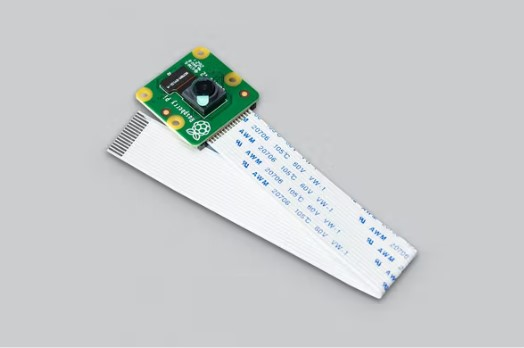
\includegraphics[width=8cm]{pics/RaspberryPiCameraModule2.jpg}
\end{figure}
\cite{PiCamera}
\subsubsection{Display}
\begin{figure}
  \centering
  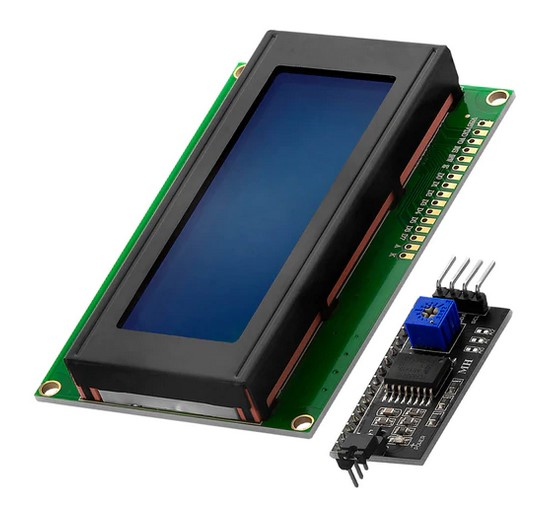
\includegraphics[width=8cm]{pics/RaspberryDisplay.jpg}
\end{figure}
\cite{RaspberryDisplay}
Um dem Nutzer vor der Garage mitzuteilen, was gerade geschieht, wird ein Display verwendet, auf dem mitgeteilt wird, ob die Kombination, welche auf dem Nummernfeld eingegeben wurde, korrekt ist, oder ob die NFC-Karte autorisiert ist.
Da auf diesem Display nur kurze Textausgaben angezeigt werden, fiel die Entscheidung auf ein LCD-Display gesetzt, welches in zwei Zeilen beschrieben werden kann. Dieses bat zudem weitere Vorteile wie die geringen Kosten von 9€ pro Stück, die Spannungsversorgung durch den Raspberry Pi selbst, sowie die einfache Möglichkeit, Text darauf auszugeben.
Im Lieferumfang des Displays war zudem ein I2C Serial Adapter, welcher durch seine 4 benötigen Ports um 8 Pins auf dem Raspberry Pi weniger benötigt, als das direkt angeschlossene Display. \\
\subsubsection{Display}
\begin{figure}
  \centering
  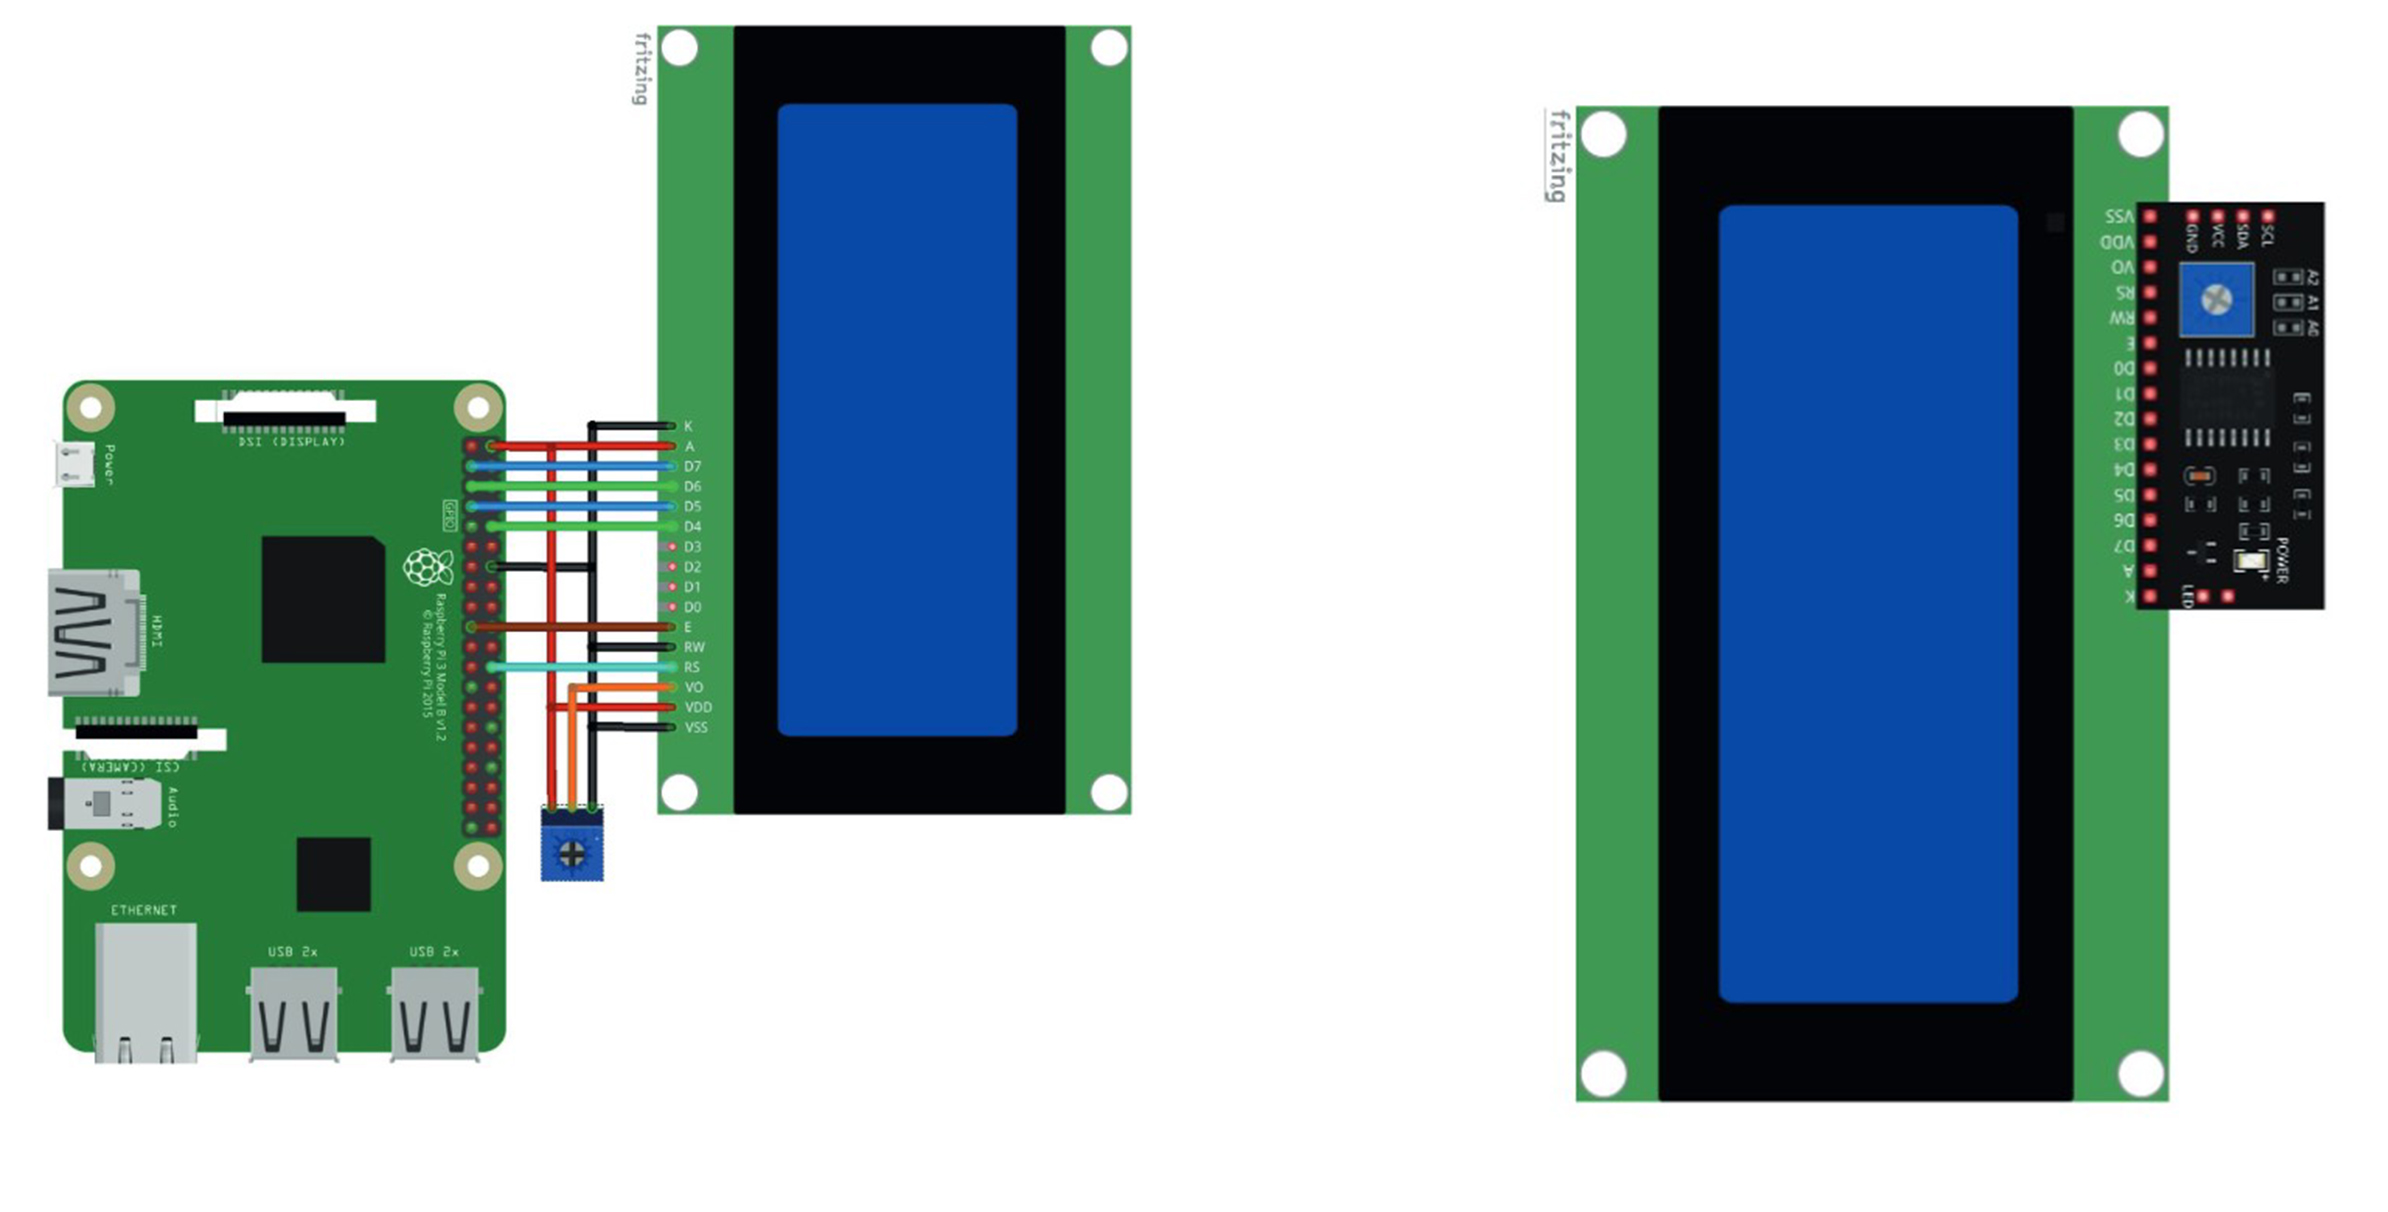
\includegraphics[width=15cm]{pics/DisplayComparison.jpg}
\end{figure}
Die technischen Daten des Displays lauten:
\begin{itemize}
  \item 4 Zeilen zu je 20 Zeichen beschreibbar
  \item Blaue Hintergrundbeleuchtung
  \item 5V Versorgungsspannung
\end{itemize}